% Please do not change the document class
\documentclass{scrartcl}

% Please do not change these packages
\usepackage[hidelinks]{hyperref}
\usepackage[none]{hyphenat}
\usepackage{setspace}
\usepackage{graphicx}
\doublespace

% You may add additional packages here
\usepackage{amsmath}

% Please include a clear, concise, and descriptive title
\title{An Analysis of the Variability, Reliability, and Control Provided by Level Generation Techniques for 2D Platform Games}

% Please do not change the subtitle
\subtitle{COMP110 - Computer Architecture Essay}

% Please put your student number in the author field
\author{1507290}

\begin{document}

\maketitle

\abstract{There are a number of diverse approaches to level generation for 2D platform games, each placing emphasis on a different aspect of level generation. Chunk-based approaches tend to favour control and variation, whilst rhythm-based approaches such as that favour playability and enjoyability. There are also evolutionary approaches that use genetic algorithms, which when combined with constraint satisfaction provide a high level of control and reliability. For an independant games developer with limited resources, generating creative, high quality levels with minimal human input is essential.}

\section{Introduction}
Procedural content generation for 2D platform games is a relatively new field in comparison to games of other genres~\cite{compton:platform}. Many diverse approaches to this problem have been developed, each with different characteristics~\cite{horn:comparative}. There are chunk-based approaches which rely on hand-designed chunks of level; rhythm-based models that generate a level based on sequences of player actions; and evolutionary approaches that use genetic algorithms. For an independent games company who desire creative control yet do not posess the time or resources to hand design a large amount of levels, the most desirable level generator would be one that requires minimal human input yet offers a high level of control and generates a wide variety of fun and playable levels consistently. 

\section{Comparison}

\subsection{Overview}
Smith et al.~\cite{smith:launchpad} base their level generation tool, Launchpad, on the concept of rhythm. They define rhythm as being the ideal sequence and timing of button presses that the player must execute; for example, a series of jumps. They use a two-tiered, grammar-based approach, where rhythm is generated separately, ensuring it is always present regardless of the level geometry.
\begin{figure}[h]
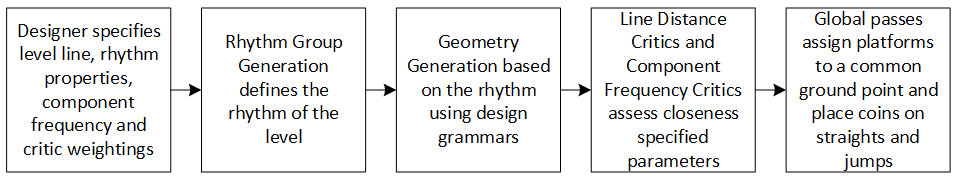
\includegraphics[width=\textwidth]{figs/launchpad.png}
\caption{Launchpad's Level Generation Process}
\end{figure}

Sorenson et al.~\cite{sorenson:generic} are also inspired by rhythm with their technique, but instead define rhythm as alternating periods of high and low difficulty. They use a genetic algorithm to generate levels. The quality of a level is determined by a fitness function, and levels that have a high fitness value are able to pass their genetic information on to future generations, resulting in levels gradually being improved. They also use constraint satisfaction to ensure playability and provide additional control. Although other approaches using evolutionary algorithms have been developed~\cite{mourato:genetic}, Sorenson et al.'s offers more direct control. Furthermore, the algorithm has been designed to be general and able to apply to any genre of game.
\begin{figure}[h]
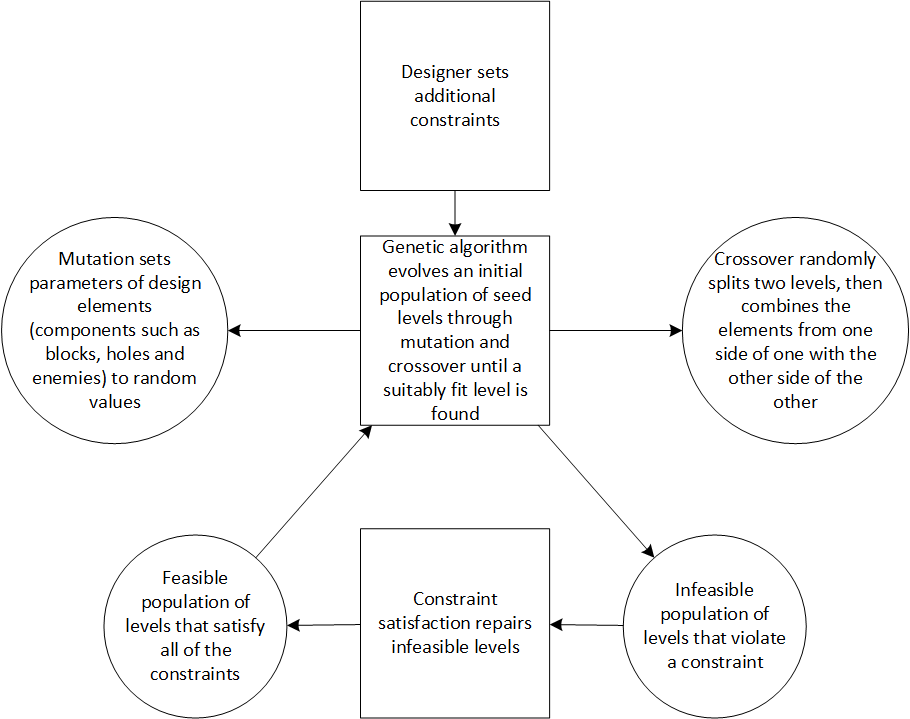
\includegraphics[width=\textwidth]{figs/genetic.png}
\caption{Sorenson et al.'s Level Generation Process}
\end{figure}


Mawhorter and Mateas~\cite{mawhorter:occupancy} take a different approach to level generation with Occupancy-Regulated Extension (ORE). Instead of levels being generated from individual components, ORE uses pre-authored chunks of level and stitches them together based on anchor points that represent places the player can occupy. Unlike the other two algorithms, the system has no strict measures in place to ensure playability as it was designed to prioritise variability.

\begin{figure}[h]
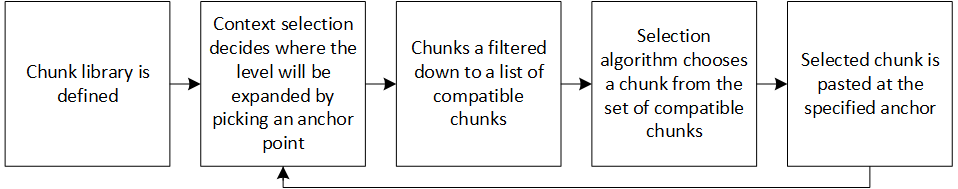
\includegraphics[width=\textwidth]{figs/ore.png}
\caption{Level Generation Process using Occupancy Regulated Extension}
\end{figure}


\subsection{Human Input and Control}
Launchpad is designed to require minimal effort whilst offering high levels of control. It allows the rhythm, the path of the level, and the desired number of each component to be specified. A number of levels are generated and assessed before a pool of the best matches is presented to the designer. In practice, this means that Launchpad may be better for aiding the design of levels, rather than generating them in-game. Even if the closest matching level could automatically be chosen, generating a large pool of levels would make the process take longer with no visible results.

Sorenson et al.'s approach also allows the number of each design element to be restricted. Additionally, the designer can adjust the difficulty of the generated levels by changing one parameter. If desired, part of the level can be hand-designed and the rest of the level generated around it. This means that level profiles for each part of the game could be specified, allowing control over progression whilst maintaining variation. This could even be used to adapt the levels to the player, by reducing the difficulty parameter if the player repeatedly loses. This provides a high level of creative control to the designer with little required effort.

Of the three methods, ORE requires the most human effort. Level chunks must be hand-authored, meaning that the output is greatly influenced by the quality of the chunks. Additionally, in order to achieve the desired result, an understanding of how the algorithm works is required. One advantage of hand designing chunks, however, is that chunks can be of any nature, allowing more complex structures to be generated.


\subsection{Flexibility and Variability}
Smith et al. claim that their two-tiered approach allows a wide variety of levels to be produced. That is, levels with the same rhythm can have many variations. Certain patterns and tendencies can be observed in the levels generated by Launchpad, however. The levels tend to be very linear and have little pattern variation~\cite{horn:comparative}. This means that the generated levels may begin to feel repetitive after extended play time. Additionally, the emphasis on rhythm means that the generated levels are only appropriate for dexterity based platform games.

This is also an issue with Sorenson et al.'s algorithm, as the model of fun used in the fitness function is based around challenge and difficulty with respect to skill. On the other hand, there is the scope to adjust the fitness function. If required, a fitness function based on a different model of fun could be developed, to allow levels suitable for other types of platform games to be generated. Furthermore, their implementation of rhythm is looser, allowing levels to be less linear and repetitive. This results in more interesting and varied levels.

ORE could potentially generate levels appropriate for other types of platform games, such as those that focus on exploration. This would be possible as chunks can be designed with any desired result in mind, whilst the algorithm does not need adjusting since the playability of levels is not assessed. Additionally, much variation in patterns on the generated levels can be observed~\cite{horn:comparative}, which could have a positive impact the fun and replayability of levels generated by ORE. This is offset by the large amount of work required to use ORE effectively.


\subsection{Playability and Design}
Launchpad and Sorenson et al.'s approach have comprehensive algorithms in place to ensure playability. Launchpad has a physics engine that is aware of the movement speed and jump height of the player, which is used when generating the level geometry to ensure that the resulting level is possible to complete.
Sorenson et al. specify the requirements for playability in the form of constraints, meaning that unplayable levels are repaired using constraint satisfaction before being returned to the population of acceptable levels. 
ORE focus on variability means that it has no measures in place to guarantee playability. This reduces the possible applications of ORE, as it would be risky to use it to generate levels in-game in case the player is presented with an unbeatable level. One option is to use an additional algorithm to determine whether the level is playable before presenting it to the player, but that would use additional resources and extend the time taken.

Smith et al. and Sorenson et al. also ensure that the levels are fun. Both of their definitions of fun are inspired by the concept of 'flow' as described by Csikszentmihalyi~\cite{csik:flow, smith:rhythm}. The fitness function used in Sorenson et al.'s genetic algorithm is based on their comprehensive model of fun~\cite{sorenson:fun}, ensuring that the population evolves towards 'fun' levels. Smith et al. apply their definition of fun in the algorithm that generates the rhythm groups. Although 'fun' is subjective, these two algorithms ensure that at least some form of theoretical 'fun' will be present in the game.
ORE is not based on any model of fun. The enjoyability of the resulting level depends both on how well the chunks have been designed and the implementation of the chunk selection algorithm. Again, this puts a lot of emphasis on the designer. With chunks designed by the authors of the algorithm, ORE came fourth in the \textit{2010 Mario AI Championship}~\cite{shaker:mario}, whilst Sorenson et al. managed to place third, despite their approach being generalised.


\section{Conclusion}
Whilst ORE provides great control over the design of a generated level, Launchpad and Sorenson et al.'s approach provide greater flexibility and reliability with little effort. Sorenson et al.'s approach perhaps provides greater control and flexibility than launchpad; parameters are able to easily be altered and level sections can be designed by hand, in addition to providing control over component numbers. They have comprehensively modeled the concept of 'fun' and ensured that all levels generated comply with it. Its success is demonstrated by their reasonable placing in the \textit{2010 Mario AI Championship}~\cite{shaker:mario}, despite being a general approach. Overall, Sorenson et al.'s approach would allow a small independent developer to reliably produce fun and playable levels with minimal effort, whilst providing a high level of creative control.


\bibliographystyle{ieeetr}
\bibliography{comp110_architecture}

\end{document}
